%%%%%%%%%%%%%%%%%%%%%%%%%%%%%%%%%%%%%%%%%
% Beamer Presentation
% LaTeX Template
% Version 1.0 (10/11/12)
%
% This template has been downloaded from:
% http://www.LaTeXTemplates.com
%
% License:
% CC BY-NC-SA 3.0 (http://creativecommons.org/licenses/by-nc-sa/3.0/)
%
%%%%%%%%%%%%%%%%%%%%%%%%%%%%%%%%%%%%%%%%%

%-------------------------------------------------------------------------------
%	PACKAGES AND THEMES
%-------------------------------------------------------------------------------

%\documentclass{beamer}
\documentclass[12pt, aspectratio=169]{beamer}
\usepackage{keynote-gradient}

\mode<presentation> {

% The Beamer class comes with a number of default slide themes
% which change the colors and layouts of slides. Below this is a list
% of all the themes, uncomment each in turn to see what they look like.

%\usetheme{default}
%\usetheme{AnnArbor}
%\usetheme{Antibes}
%\usetheme{Bergen}
%\usetheme{Berkeley}
%\usetheme{Berlin}
%\usetheme{Boadilla}
%\usetheme{CambridgeUS}
%\usetheme{Copenhagen}
%\usetheme{Darmstadt}
%\usetheme{Dresden}
%\usetheme{Frankfurt}
%\usetheme{Goettingen}
%\usetheme{Hannover}
%\usetheme{Ilmenau}
%\usetheme{JuanLesPins}
%\usetheme{Luebeck}
%\usetheme{Madrid}
%\usetheme{Malmoe}
%\usetheme{Marburg}
%\usetheme{Montpellier}
%\usetheme{PaloAlto}
%\usetheme{Pittsburgh}
%\usetheme{Rochester}
%\usetheme{Singapore}
%\usetheme{Szeged}
%\usetheme{Warsaw}

% As well as themes, the Beamer class has a number of color themes
% for any slide theme. Uncomment each of these in turn to see how it
% changes the colors of your current slide theme.

%\usecolortheme{albatross}
%\usecolortheme{beaver}
%\usecolortheme{beetle}
%\usecolortheme{crane}
%\usecolortheme{dolphin}
%\usecolortheme{dove}
%\usecolortheme{fly}
%\usecolortheme{lily}
%\usecolortheme{orchid}
%\usecolortheme{rose}
%\usecolortheme{seagull}
%\usecolortheme{seahorse}
%\usecolortheme{whale}
%\usecolortheme{wolverine}

%\setbeamertemplate{footline} % To remove the footer line in all slides uncomment this line
\setbeamertemplate{footline}[page number] % To replace the footer line in all slides with a simple slide count uncomment this line

\setbeamertemplate{navigation symbols}{} % To remove the navigation symbols from the bottom of all slides uncomment this line
}

\usepackage{graphicx} % Allows including images
\usepackage{booktabs} % Allows the use of \toprule, \midrule and \bottomrule in tables

%-------------------------------------------------------------------------------
%	TITLE PAGE
%-------------------------------------------------------------------------------

\title[HSE research proposal]{iPavlov research proposal: \\Neuromorphic breakthrough directions} % The short title appears at the bottom of every slide, the full title is only on the title page

\author[Max Talanov]{
  Max Talanov
} 
\institute[for: iPavlov] % Your institution as it will appear on the bottom of every slide, may be shorthand to save space
{
for iPavlov \\ % Your institution for the title page
\medskip
\textit{max.talanov@gmail.com} % Your email address
}
\date{\today} % Date, can be changed to a custom date

\begin{document}

\begin{frame}
\titlepage % Print the title page as the first slide
\end{frame}


%-------------------------------------------------------------------------------
%	PRESENTATION SLIDES
%-------------------------------------------------------------------------------

%------------------------------------------------
\section{Emotions}
%------------------------------------------------

\begin{frame}
\frametitle{\#1 Emotions}
\begin{columns}[c] % The "c" option specifies centered vertical alignment while the "t" option is used for top vertical alignment

\column{.45\textwidth} % Left column and width

\begin{itemize}
\item Bio-plausible emotional drives
\item Integrated with niciception and reward systems (DA)
\item Integrated with motor output brain stem and spinal cord
\end{itemize}

\column{.6\textwidth} % Right column and width
%------------------------------------------------
\begin{figure}
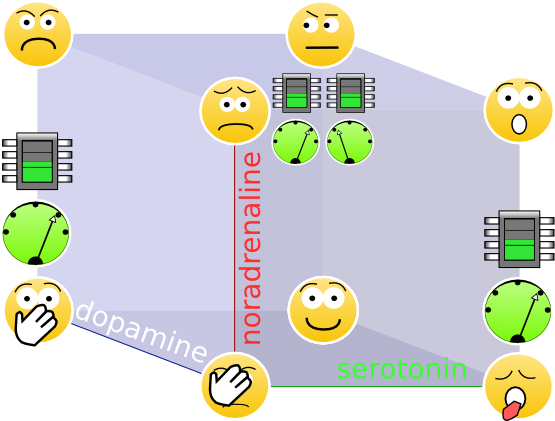
\includegraphics[width=0.8\linewidth]{cube_of_emotional_parameters_machine}
\end{figure}
%------------------------------------------------
\end{columns}
\end{frame}

%------------------------------------------------
%------------------------------------------------

\begin{frame}
\frametitle{Emotional drives}
\begin{itemize}
 \item \emph{Computing utilization} is a metric to quantify how busy the processing resources of the system are. It is expressed by the average value of all the single processing resources' utilization.
 \item \emph{Computing distribution} quantifies the load balancing among processing resources. It is expressed as the variance of single resources' utilization.
 \item \emph{Memory distribution} is associated with the amount of memory allocated to the processing resources. It is quantified by the variance of the amount of memory per single resource.
 \item \emph{Storage volume} is an index related to the the amount of data and information used by the system.
 \item \emph{Storage bandwidth} quantifies the number of connections between resources, i.e. processing and data nodes.
% persistence of data and information.
\end{itemize}
\end{frame}

%------------------------------------------------
\subsection{DA}
%------------------------------------------------

\begin{frame}
\frametitle{Emotions: dopamine (DA) subsystem}
\begin{figure}
\includegraphics[width=0.8\linewidth]{dopamine_diagram}
\end{figure}
\end{frame}

%------------------------------------------------
%------------------------------------------------

\begin{frame}
\frametitle{DA results: fear-like}
\begin{figure}
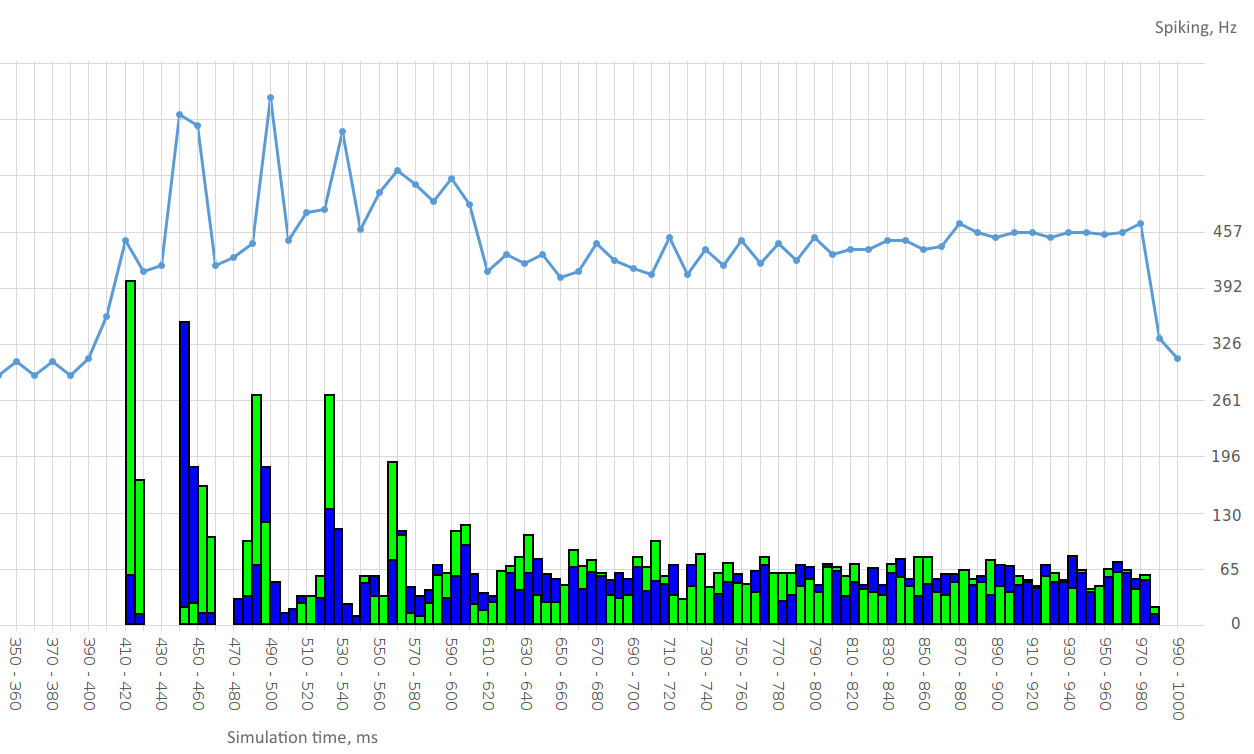
\includegraphics[width=0.6\linewidth]{resultBIG_short}
\end{figure}
400 - 600 ms - simulated brain in placed in the ``fear-like'' state that is indicated with increased level of neuronal activity on motor cortex and thalamus as well as increased computational power consumption.
\end{frame}

%------------------------------------------------
\subsection{5HT}
%------------------------------------------------

\begin{frame}
\frametitle{Emotions: serotonin (5HT) subsystem}
\begin{figure}
\includegraphics[width=0.7\linewidth]{serotonin_diagram}
\end{figure}
\end{frame}

%------------------------------------------------
%------------------------------------------------

\begin{frame}
\frametitle{5HT results: disgust-like}
\begin{figure}
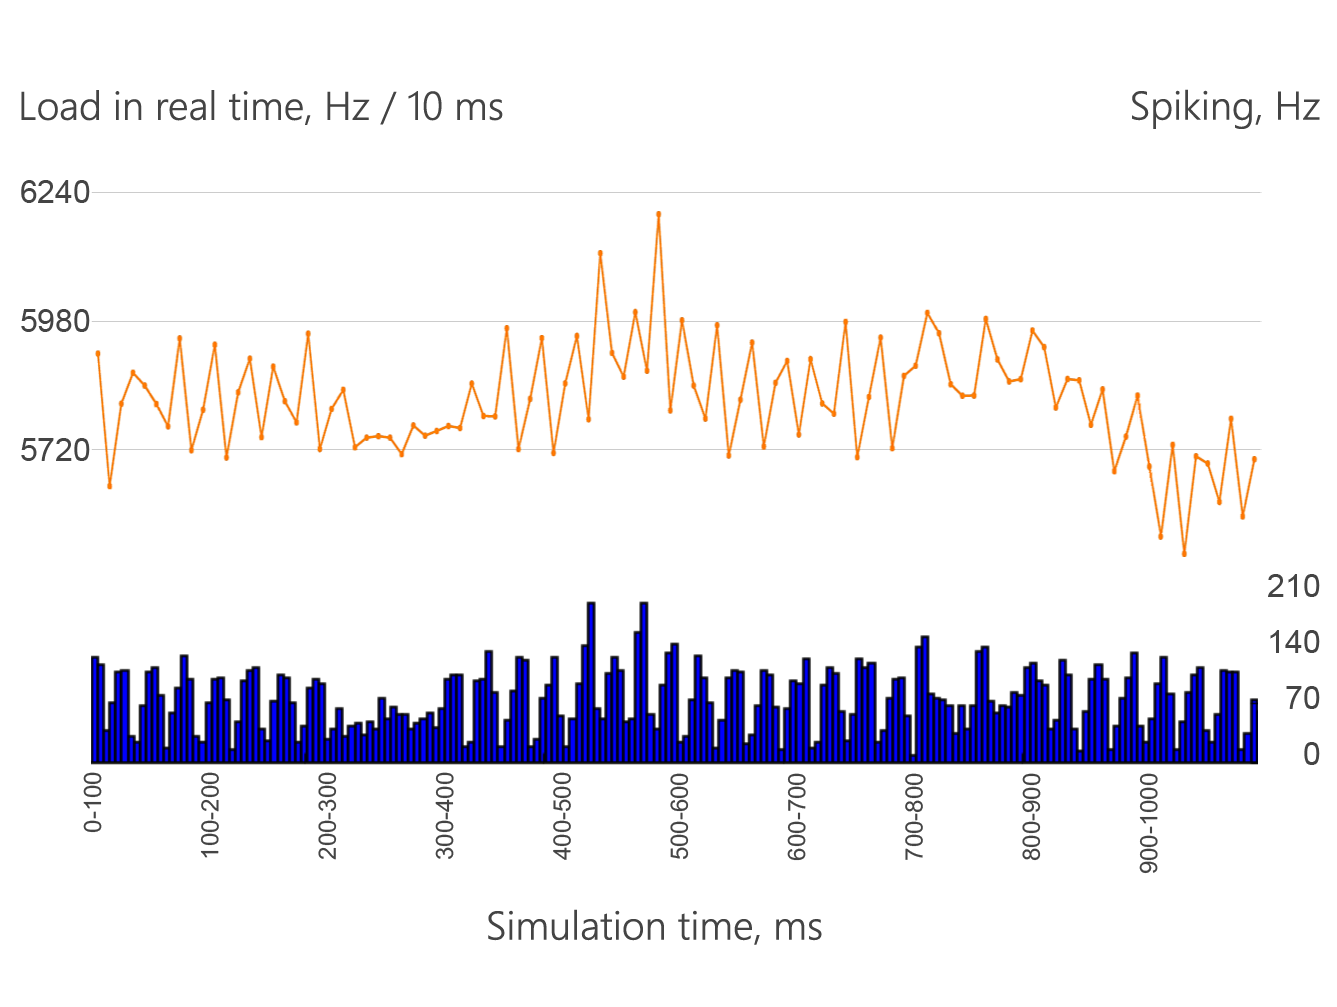
\includegraphics[width=0.6\linewidth]{5ht_results}
\end{figure}
200 - 300 simulated brain in placed in the ``disgust-like'' that is indicated with decreased level of neuronal activity on motor cortex and computational power.
\end{frame}

%------------------------------------------------
\subsection{NA}
%------------------------------------------------

\begin{frame}
\frametitle{Emotions: noradrenaline (NA) subsystem}
\begin{figure}
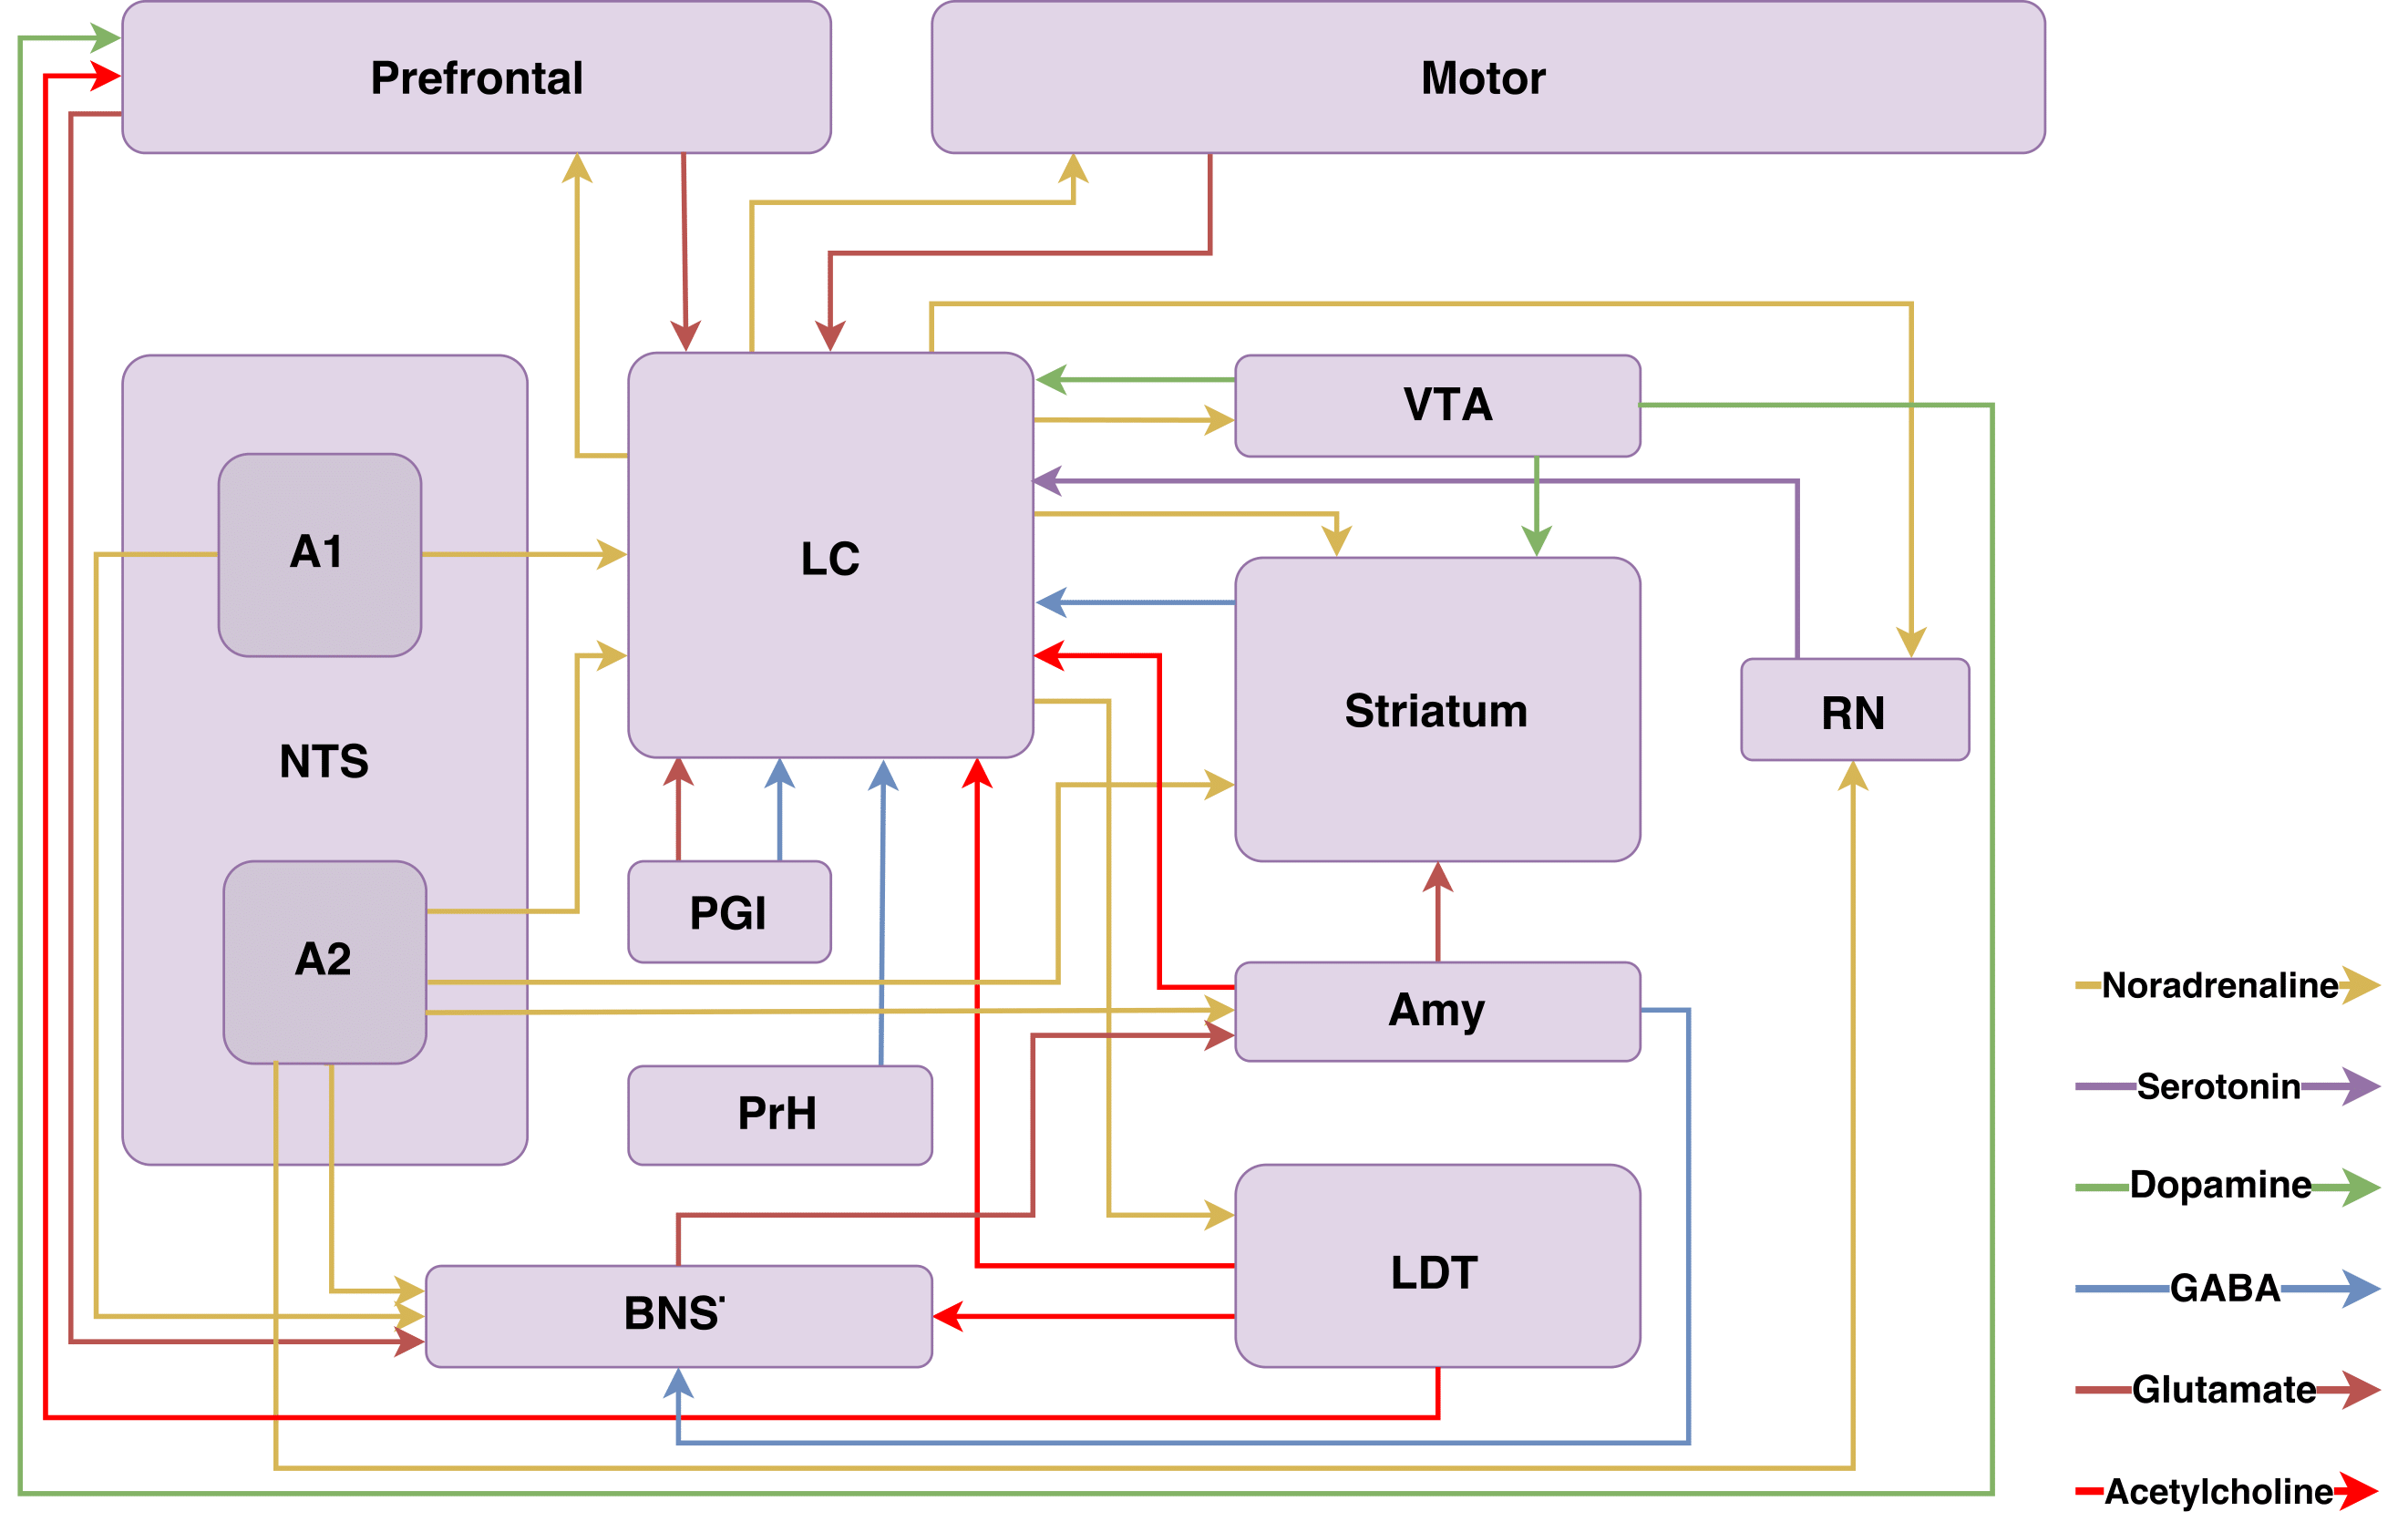
\includegraphics[width=0.7\linewidth]{na_diagram}
\end{figure}
\end{frame}

%------------------------------------------------
\section{Memristive brain (new hardware)}
%------------------------------------------------

\begin{frame}
\frametitle{\#2 Memristive brain (hardware)}
\begin{figure}
\includegraphics[width=0.8\linewidth]{HL_Emristor}
\end{figure}
\end{frame}

%------------------------------------------------

\begin{frame}
\frametitle{Memristive brain}
  
Inputs $1, ..n, ..n + m$ where n is the number of excitatory synapses and m is number of inhibitory synapses per one cell. The scale of the n+m is $10^4$.

Excitatory memristive elements are trained via Hebbian learning, inhibitory memristive elements are trained via ``sombrero''. The adder implements balancing of excitatory and inhibitory impact of memristive elements (synapses), and its output starts the output impulse (spike) generator. The inverting adder to be compared with integrated input of the neuron provided and extended via the integrator 1. The inverting adder output is transmitted to inhibitory memristive elements and implements ``sombrero'' training. The monostable multivibrator is activated via positive signal of the inverting adder triggering a relay that grounds the slave inverter crating the positive half of $\Delta t$ axis of the learning function graph. The negative half of the graph is created via the slave inverter in the non-grounded mode. The output of the feedback: $\frac{1}{x}$ or Hebbian learning is transferred to excitatory memristive elements.
  
\end{frame}

%------------------------------------------------
\section{Integration and Robot dream}
%------------------------------------------------

\begin{frame}
\frametitle{\#3 Integration and Robot dream}
\begin{figure}
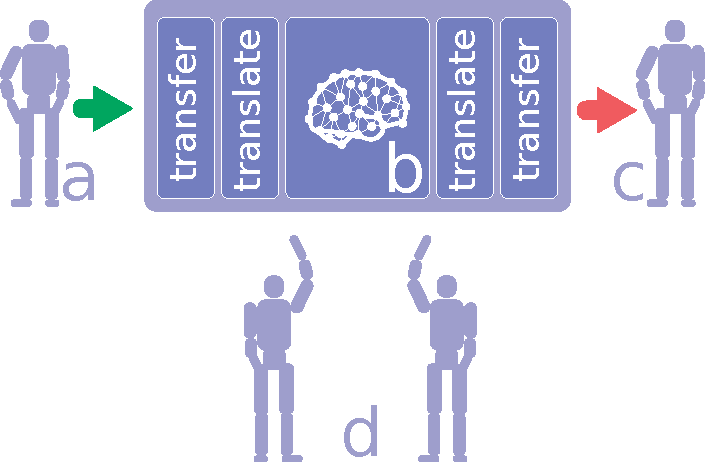
\includegraphics[width=0.8\linewidth]{robot-dream}
\end{figure}
\end{frame}

%------------------------------------------------
\section{Future work}
%------------------------------------------------

\begin{frame}
  \frametitle{Future work}
  
\begin{itemize}
  \item Simple prototype as feasibility study.
  \item \ldots\
  \item Emotional robot with real-time embodiment
  \item Social robot with emotions
  \item Conscious social robot
\end{itemize}

\end{frame}

%------------------------------------------------
%------------------------------------------------

\end{document} 
